\section{Results}\label{sec:results}

We evaluate the method on three Alpine glaciers of contrasting size---Argentière,
Great Aletsch and Rhône---each processed through the same glacier-agnostic two-step
pipeline: the data assimilation inverts the ice thickness while the basal-motion
parameter $\tau_{\mathrm{ref}}$ is fixed by an ensemble search to the scalar that
minimises the surface-velocity misfit, after which the $smb$ is inferred. No
per-glacier retuning of the regularisation, optimiser or parametrisation is applied,
and none of the three uses a thickness survey. Argentière additionally carries the
state-of-the-art distributed reconstruction of \citet{kneib2024}, against which we
compare our velocity-only result directly.


\subsection{Calibrated ice-dynamics states}\label{sec:calib}

For every glacier the data assimilation converges within $\mathcal{O}(10^2)$ L-BFGS
iterations to a thickness field whose modelled surface velocity matches the
observations to a root-mean-square residual of a few $\mathrm{m\,yr^{-1}}$---$2.4$ on
Argentière, $11$ on Great Aletsch and $6.8$ on Rhône at the adopted
$\tau_{\mathrm{ref}}$---one to two orders of magnitude
below typical trunk velocities (locally exceeding
$100$--$150\,\mathrm{m\,yr^{-1}}$). The calibrated state fixes the bedrock through
Eq.~\eqref{eq:bed} and provides the starting geometry $H_{t_1}$ for the transient
forward run (Sect.~\ref{sec:inference}).

Figure~\ref{fig:da-state} shows the calibrated state on Argentière: the recovered
ice-thickness field (a), and the close match between the observed (b) and modelled
(c) surface speed, whose differences are small and spatially unstructured.

\begin{figure*}
  \centering
  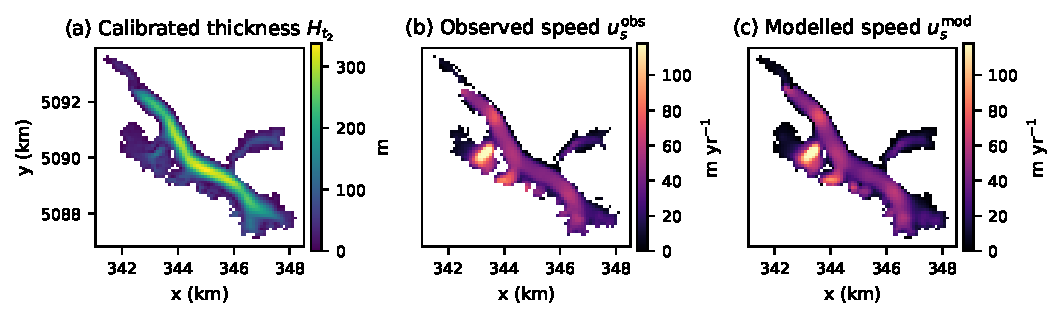
\includegraphics[width=\linewidth]{figs/fig_da_state.pdf}
  \caption{Calibrated data-assimilation state on Argentière at the start epoch,
    for the adopted velocity-only run
    ($\tau_{\mathrm{ref}}=0.27\,\mathrm{MPa}$).
    (a)~Calibrated ice thickness $H_{t_1}$; (b)~observed surface speed
    $u_s^{\mathrm{obs}}$ \citep{millan2022}; (c)~modelled surface speed
    $u_s^{\mathrm{mod}}$, in close agreement with the observations.}
  \label{fig:da-state}
\end{figure*}

As a final check, we confirm the calibrated state is free of the initialisation
shock of Sect.~\ref{sec:overview}: integrated forward for one year under zero $smb$,
it produces no spurious thickness drift, so the glacier is in mechanical equilibrium
and any subsequent geometry change is attributable to the prescribed $smb$ rather
than to residual model imbalance.

\subsection{Inferred SMB and validation}\label{sec:inferred}

Holding the calibrated state ($H_{t_1}$, $\tau_{\mathrm{ref}}$, $A$) fixed, we run the
transient forward simulation over each glacier's window and invert for the
elevation-resolved $smb$ profile $smb(z)$ that minimises the geometry-misfit cost
(Eq.~\ref{eq:cost}). On all three glaciers the retrieved profile increases
monotonically across the full altitudinal range, from strongly negative values at
the tongue to a positive accumulation regime in the upper basin.

On Argentière (2012--2021) the profile reproduces the observed altitudinal pattern
of the GLACIOCLIM stakes with a root-mean-square error of
$0.65\,\mathrm{m\,w.e.\,yr^{-1}}$ (Fig.~\ref{fig:smb-continuity}a,
Table~\ref{tab:rmse}). This is obtained with the generic velocity-only
pipeline---no thickness survey, no per-glacier tuning, no \emph{post hoc}
smoothing---yet it is on par with the best physically-based reconstructions of
\citet{kneib2024} on the same stakes, whose SIA and IGM-distributed approaches give
$0.67$ and $0.85\,\mathrm{m\,w.e.\,yr^{-1}}$ and whose flux-gate F2019 estimate
gives $0.50$, all of which additionally require ice-thickness
data. Argentière is also covered by accurate GPR thickness soundings; repeating the
experiment with them---inverting $\tau_{\mathrm{ref}}$ as a spatial field---lowers
the error further and surpasses every published reconstruction on this site, as
detailed in Appendix~A1. Because the inversion variable is one-dimensional,
horizontal heterogeneity within an elevation band---notably the avalanche-fed
accumulation hotspots reported by \citet{kneib2024}---is not resolved; this
deliberate trade-off, which buys a tuning-free and transferable inversion, is taken
up in Sect.~\ref{sec:discussion}.

\begin{table}
    \centering
    \caption{Validation of the inferred SMB against the GLACIOCLIM stake network on
    Argentière Glacier (main trunk + Améthystes tributary) over 2012--2021. The
    three baselines are the modelling approaches of \citet{kneib2024}, evaluated
    against the same stakes; all three use ice-thickness data, whereas our result
    uses surface velocity only. The GPR-assisted field inversion, which improves
    further on these, is reported in Appendix~A1.}
    \label{tab:rmse}
    \begin{tabular}{lc}
        \hline
        Method & RMSE [m\,w.e.\,yr$^{-1}$] \\
        \hline
        F2019 \citep{kneib2024}                       & 0.50 \\
        SIA \citep{kneib2024}                          & 0.67 \\
        IGM-distributed \citep{kneib2024}              & 0.85 \\
        \textbf{Ours (velocity only, scalar $\tau_{\mathrm{ref}}$)} & \textbf{0.65} \\
        \hline
    \end{tabular}
\end{table}

The same pipeline, applied without modification to Great Aletsch (2009--2017) and
Rhône (2007--2016), yields equally smooth, monotonic profiles that reproduce the
independent stake averages---two continuous-record locations on Aletsch and five on
Rhône (Sect.~\ref{sec:data})---with root-mean-square errors of $0.61$ and
$0.32\,\mathrm{m\,w.e.\,yr^{-1}}$ (Fig.~\ref{fig:smb-continuity}b,c). 
These are on par with the Argentière result despite the absence of any thickness
constraint, which we read less as a
coincidence than as evidence that the velocity-calibrated dynamical
state carries the elevation structure of the SMB; whether the robustness holds
across a larger and more varied sample than three large glaciers is an open question
we return to in Sect.~\ref{sec:discussion}.

\begin{figure*}
  \centering
  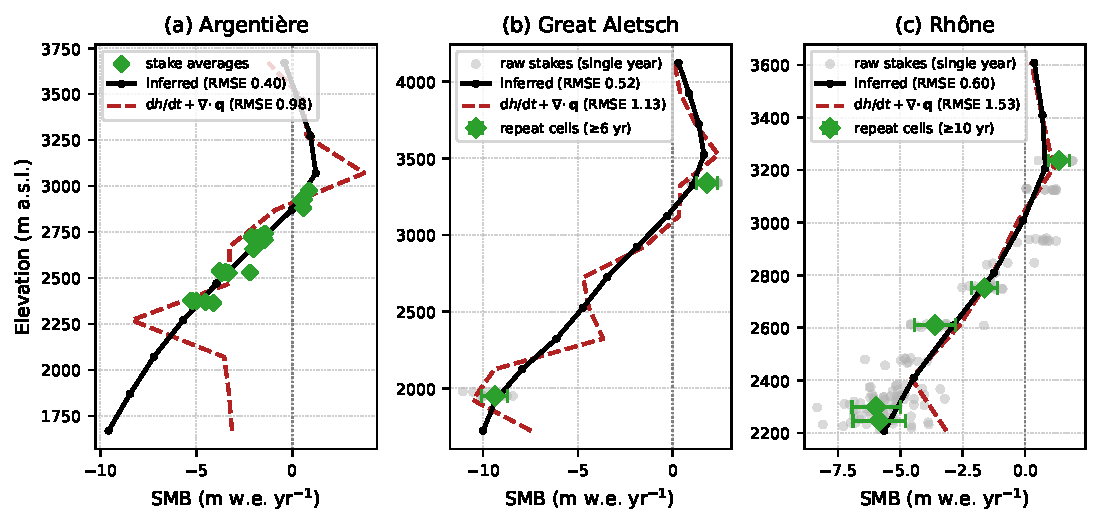
\includegraphics[width=\linewidth]{figs/fig_continuity_3panel.pdf}
  \caption{Inferred SMB profile (black) for (a)~Argentière, (b)~Great Aletsch and
    (c)~Rhône, compared against in situ stake measurements and against the continuity
    estimate $\mathrm{d}h/\mathrm{d}t + \nabla\!\cdot\mathbf{q}$ (dashed) obtained with
    the \emph{stationary} data-assimilation flux divergence. Green diamonds are the
    continuous-record stake averages ($\pm$ interannual standard deviation), the
    validation targets (faint grey dots on Aletsch and Rhône are the raw single-year
    readings). The inferred profile tracks the averages across the whole elevation
    range ($\mathrm{RMSE}=0.65$, $0.61$ and $0.32\,\mathrm{m\,w.e.\,yr^{-1}}$),
    whereas the stationary-flux estimate departs strongly in the ablation zone
    ($2.14$, $1.59$ and $1.63$).}
  \label{fig:smb-continuity}
\end{figure*}

Figure~\ref{fig:smb-continuity} makes concrete the
mass-conservation argument of Sect.~\ref{sec:sota}. The dashed curve is the SMB the
continuity equation yields when the flux divergence is taken as stationary, exactly
as in flux-divergence inversions. On every glacier this estimate is markedly noisier
than the inferred profile and diverges in the ablation zone, where the stationary
divergence is least representative, raising the stake RMSE to $2.14$ (Argentière),
$1.59$ (Aletsch) and $1.63\,\mathrm{m\,w.e.\,yr^{-1}}$ (Rhône)---a factor of $2.6$ to
$5$ worse than our transient inversion. Because our forward model integrates the
mass-conservation law directly and recomputes the flux divergence from the evolving
geometry at every step, the inferred profile requires no spatial smoothing and
remains mass-consistent throughout.

\subsection{Sensitivity to the basal-motion parameter}\label{sec:sensitivity}

The basal-motion parameter $\tau_{\mathrm{ref}}$ is the dynamical quantity least
constrained on a glacier without thickness or stake data, where its value rests on
the surface-velocity misfit (\emph{velsurf}) alone. It is also intrinsically hard to
separate from the ice thickness: a more slippery bed (smaller $\tau_{\mathrm{ref}}$)
inferred together with thinner ice reproduces almost the same surface
velocity---and hence the same ice flux---as a stiffer bed carrying thicker ice, so
many $(\tau_{\mathrm{ref}}, H)$ pairs fit the observations nearly equally well. For
the $smb$ inversion this ambiguity is not fatal, because what drives the geometry
change is not the pair itself but the flux divergence $\nabla\!\cdot\mathbf{q}$ it
produces. To see how the residual freedom in $\tau_{\mathrm{ref}}$ propagates into the
inferred $smb$, we repeated the $smb$ inversion across a wide range of
$\tau_{\mathrm{ref}}$ on all three glaciers (Fig.~\ref{fig:sens}), using the
independent stake RMSE as ground truth against \emph{velsurf}, the only selector
available operationally.

\begin{figure*}
  \centering
  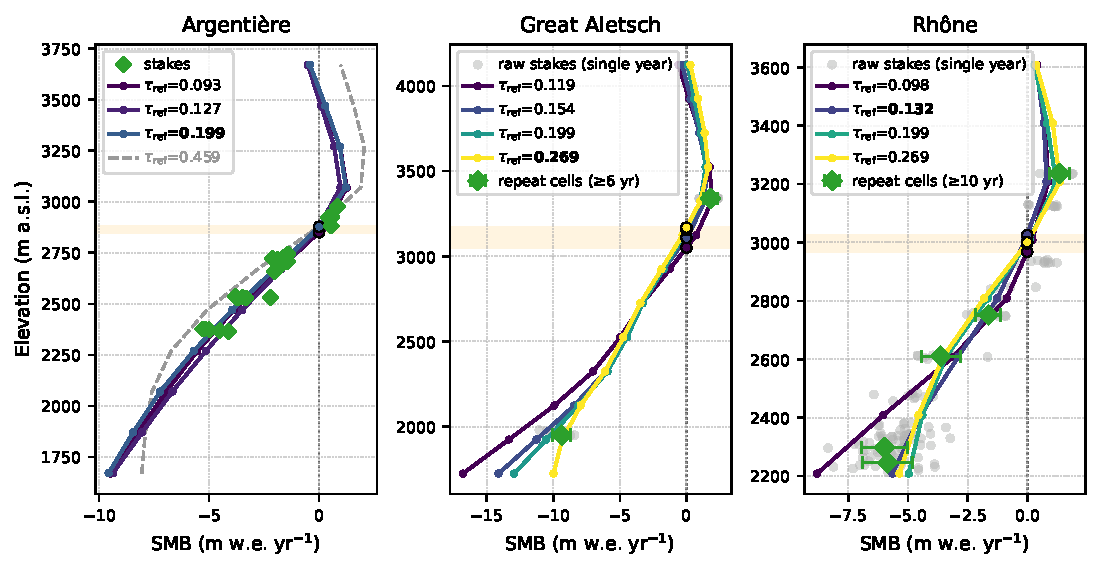
\includegraphics[width=\linewidth]{figs/sens_slidingco_3panel.pdf}
  \caption{Inferred SMB profiles across a range of the basal-motion parameter
    $\tau_{\mathrm{ref}}$ for (a)~Argentière, (b)~Great Aletsch and (c)~Rhône;
    colour encodes $\tau_{\mathrm{ref}}$ and the adopted profile is drawn bold.
    Within the low-velocity-misfit basin the profiles coincide in the accumulation
    area and diverge only at the ablation tongue, so the residual uncertainty in
    $\tau_{\mathrm{ref}}$ translates into an equilibrium-line-altitude band (shaded)
    rather than a whole-profile bias; the runs the velocity misfit rejects (dashed)
    depart most strongly.}
  \label{fig:sens}
\end{figure*}

Two features stand out. First, \emph{velsurf} reliably rejects the strongly biased
runs: the profiles that depart most from the stakes are also those with the worst
velocity misfit (Fig.~\ref{fig:sens}). Pooled across the three glaciers, higher
velocity misfit goes with higher stake error (Fig.~\ref{fig:corr}; Pearson $r=0.69$,
$p<10^{-2}$). Second, once these high-misfit runs are removed, the surviving
low-\emph{velsurf} runs no longer map one-to-one onto stake error: because a wide
range of $(\tau_{\mathrm{ref}}, H)$ pairs share nearly the same flux, velocity cannot
single out one value of $\tau_{\mathrm{ref}}$, and on Rhône the stake RMSE even varies
non-monotonically among them ($0.32$--$1.25\,\mathrm{m\,w.e.\,yr^{-1}}$). Crucially,
this residual freedom is confined to the ablation zone: across the low-misfit runs
the accumulation-area profile is essentially unchanged, and only the tongue
$smb$---and with it the equilibrium-line altitude---shifts from run to run
(Fig.~\ref{fig:sens}).

\begin{figure}
  \centering
  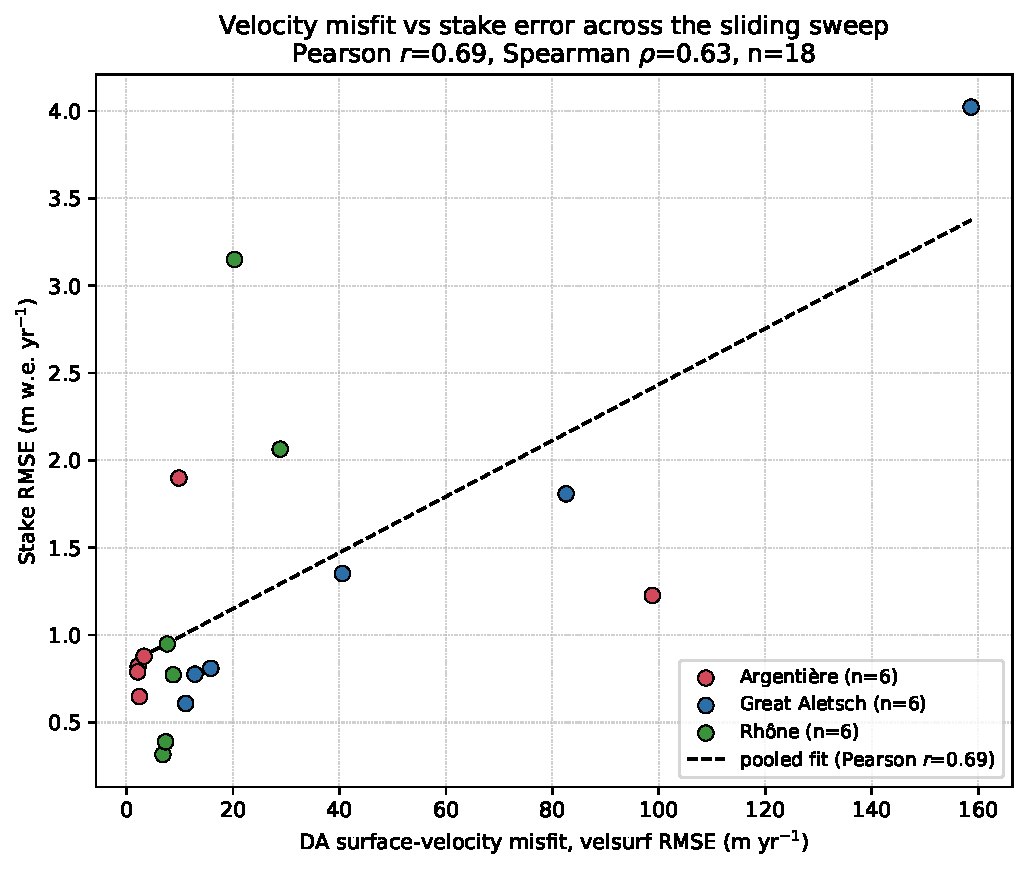
\includegraphics[width=0.6\linewidth]{figs/velsurf_vs_stake_rmse.pdf}
  \caption{Data-assimilation surface-velocity misfit (\emph{velsurf} RMSE) against
    the independent stake RMSE, pooled over the $\tau_{\mathrm{ref}}$ sweep (six
    runs per glacier, all three glaciers). Higher velocity misfit is associated with
    higher stake error (Pearson $r=0.69$, Spearman $\rho=0.63$),
    so the velocity misfit---the only selector available without stakes---carries
    usable information about the accuracy of the inferred SMB.}
  \label{fig:corr}
\end{figure}

The practical consequence is that the method does not deliver a single ``best''
profile but a family of low-\emph{velsurf} solutions that converge to the same
accumulation-area gradient and fan out only at the tongue
(Fig.~\ref{fig:sens}, Fig.~\ref{fig:corr}). For a stake-free glacier this family is
the result: the low-misfit runs together define an $smb$ and equilibrium-line
uncertainty band---narrow in the accumulation area, widening towards the tongue. How
this band behaves at regional scale, and how it might be tightened, we take up in
Sect.~\ref{sec:discussion}.
